% Rapport d'avancement Dream in Orbit, 8 novembre 2026. Compilation : tectonic rapport_8_novembre_2026.tex (ou xelatex).
% Suite du rapport du 4 novembre. Les figures viennent de figures_8_novembre.py (voir l'annexe).
\documentclass[11pt,a4paper]{article}

\usepackage{fontspec}
\usepackage{unicode-math}
\setmainfont{texgyreschola}[Extension=.otf, UprightFont=*-regular, BoldFont=*-bold,
  ItalicFont=*-italic, BoldItalicFont=*-bolditalic]
\setmathfont{texgyreschola-math.otf}
\setmonofont{texgyrecursor}[Extension=.otf, UprightFont=*-regular, BoldFont=*-bold, Scale=0.9]
\usepackage{polyglossia}
\setmainlanguage{french}

\usepackage[a4paper,margin=2.3cm,top=2.2cm,bottom=2.4cm]{geometry}
\usepackage{microtype}
\usepackage{graphicx}
\usepackage{booktabs}
\usepackage{tabularx}
\usepackage{array}
\usepackage[table]{xcolor}
\usepackage{caption}
\usepackage{float}
\usepackage{enumitem}
\usepackage{tikz}
\usetikzlibrary{positioning,arrows.meta,fit,calc}
\usepackage{fancyhdr}
\usepackage[hidelinks]{hyperref}

\definecolor{bleu}{HTML}{2A78D6}
\definecolor{orange}{HTML}{EB6834}
\definecolor{encre2}{HTML}{52514E}
\definecolor{fond}{HTML}{F3F2EE}
\definecolor{trait}{HTML}{9A9890}

\captionsetup{font=small,labelfont=bf,labelsep=period,justification=justified,singlelinecheck=false}
\setlist{itemsep=2pt,topsep=4pt}
\setlength{\parskip}{4pt}
\renewcommand{\arraystretch}{1.12}
\newcommand{\code}[1]{\texttt{#1}}
\setlength{\emergencystretch}{2em}
\newcolumntype{R}{>{\raggedleft\arraybackslash}X}

\pagestyle{fancy}
\fancyhf{}
\fancyhead[L]{\small\color{encre2}Dream in Orbit, rapport d'avancement}
\fancyhead[R]{\small\color{encre2}8 novembre 2026}
\fancyfoot[C]{\small\color{encre2}\thepage}
\renewcommand{\headrulewidth}{0.4pt}

\begin{document}

\thispagestyle{plain}
\begin{center}
  {\LARGE\bfseries Dream in Orbit}\\[4pt]
  {\large Second rapport d'avancement : du 4 au 8 novembre 2026}\\[8pt]
  {\color{encre2}Max DENIS \quad·\quad 8 novembre 2026 \quad·\quad branche \code{regime-partage}, commit \code{57abd8a}}
\end{center}

\vspace{4pt}
\noindent\colorbox{fond}{\parbox{\dimexpr\linewidth-2\fboxsep}{\small
\textbf{État au 8 novembre.} Le modèle livré dans \code{poids/} reste un ensemble de 10 world models GRU (deux jeux de variables, cinq graines chacun). Sa configuration obtient 0.0826 en validation directe et 0.0885 en validation inverse, soit 0.0855 en moyenne, contre 0.0897 au 4 novembre et 0.1155 pour la prédiction constante. Trois changements expliquent ce gain : les commandes AOOO et ATTT passent par une branche dédiée au circuit NPWD2881, la correction de niveau porte sur le résidu du simulateur avec un second terme lent, et la borne de ce résidu passe de 5 à 10 à la prédiction. Deux régularisations de robustesse ont ensuite été ajoutées au prix d'environ 0.0001. La tête de régime partagée, testée en dernier, n'a pas été retenue. Les calculs tournent maintenant sur GPU T4 Kaggle : l'entraînement du modèle final prend 629 s. Le bonus pilote n'est toujours pas commencé.}}

\vspace{6pt}
Ce rapport reprend là où s'arrêtait celui du 4 novembre, auquel il renvoie pour les données, le protocole et l'architecture de base. La section 1 rappelle le point de départ et décrit le passage sur GPU. Les sections 2 à 6 suivent les cinq sessions de travail dans l'ordre, avec les essais gardés et rejetés. La section 7 présente les résultats du modèle actuel et la section 8 ce qu'il reste à faire. Les scores sont des RMSE calculées par \code{evaluate.py}, avec un point décimal. Sauf mention contraire, ce sont des ensembles complets (2 membres × 5 graines, graines 0 à 4) entraînés sur une seule période par direction.

%=====================================================================
\section{Point de départ et passage sur GPU}

\subsection{Le modèle du 4 novembre}

Au 4 novembre, le modèle faisait la moyenne de deux ensembles de cinq GRU : l'un sur les variables v1 avec du bruit sur les entrées, l'autre sur les variables v2r. Chaque GRU lit les 7 jours de \code{power\_init} avec un encodeur, puis un simulateur avance heure par heure sur le contexte seul. Une correction additive, tirée de l'écart de \code{power\_init} à la moyenne d'entraînement, s'estompe avec une demi-vie apprise. Ce modèle faisait 0.0853 en directe et 0.0940 en inverse (moyenne 0.0897).

Le rapport précédent relevait quatre points faibles : NPWD2531 et NPWD2881 prédits plus mal qu'une constante, une correction de niveau qui ne rattrapait qu'un tiers de l'écart initial, une incertitude trop étroite et une durée d'entraînement sur GPU jamais mesurée. Les sessions suivantes partent de cette liste.

\subsection{Calcul sur GPU T4 Kaggle}

Un ensemble complet dans les deux directions prenait 2957 s sur le CPU de 16 cœurs. Le script \code{outils/lancer\_kaggle.py} envoie le dépôt dans un dataset Kaggle privé, lance un noyau sur GPU T4, attend la fin et rapatrie \code{runs/}. Le code est embarqué dans le script du noyau, ce qui évite une course entre deux versions du dataset. Deux sessions peuvent tourner en parallèle.

La même configuration prend 465 s sur T4, soit 6.4 fois moins. Relancée sur GPU, la référence donne 0.0851 / 0.0941 / 0.0896, à 0.0002 près des chiffres CPU. Deux lancements identiques sur GPU donnent les mêmes scores au chiffre près : l'entraînement y est déterministe. Toutes les mesures de ce rapport viennent du GPU, sauf mention contraire. Le protocole de décision ne change pas : un essai est gardé s'il fait baisser la moyenne d'au moins 0.0015 sans dégrader aucune direction, ou d'au moins 0.0005 avec confirmation sur les graines 5 à 9.

%=====================================================================
\section{Les commandes AOOO et ATTT}

\subsection{Constat}

\code{dio/prepare.py} ne compte que les 10 commandes \code{dmop} les plus fréquentes, qui appartiennent surtout aux familles AAAA, APSF et AVVV. Les commandes AOOO et ATTT n'arrivaient au modèle que fondues dans le compte « autres ». En regardant NPWD2881 heure par heure, j'ai vu qu'il s'allume avec ATTTF321A et s'éteint avec ATTTF321D, ou dans l'heure qui précède AOOOF01D0, AOOOF15A0 et AOOOF02A1. La relation est la même dans annee1 et annee2.

Le module \code{dio/commandes.py} construit deux variables pour chaque commande AOOO ou ATTT vue au moins 20 fois à l'entraînement : une impulsion (nombre d'occurrences dans l'heure) et un état, qui vaut 1 tant que cette commande est la dernière reçue par sa famille (par exemple ATTTF321A contre ATTTF321D). Chaque variable est lue avec un décalage compris entre $-12$ et $+12$ heures, choisi comme celui qui corrèle le mieux avec NPWD2881 sur la période d'entraînement seule. La branche du modèle final lit 71 variables de ce type.

\subsection{Où brancher les commandes}

\begin{table}[!htb]
\centering\small
\caption{Session « commandes » (GPU T4, graines 0 à 4). La ligne grisée est la configuration retenue.}
\label{tab:commandes}
\begin{tabularx}{\linewidth}{l X r r r}
\toprule
 & Changement & Directe & Inverse & Moyenne \\
\midrule
Réf. & modèle du 4 novembre, relancé sur GPU & 0.0851 & 0.0941 & 0.0896 \\
G1 & commandes AOOO en entrée du GRU & 0.0802 & 0.0966 & 0.0884 \\
G1b & commandes AOOO dans une branche à part, vers NPWD2881 seul & 0.0842 & 0.0918 & 0.0880 \\
G2 & AOOO + ATTT en entrée du GRU & 0.0819 & 0.0951 & 0.0885 \\
\rowcolor{fond} \textbf{G2b} & \textbf{AOOO + ATTT dans la branche vers NPWD2881 (retenu)} & \textbf{0.0832} & \textbf{0.0914} & \textbf{0.0873} \\
G3b & G2b + commandes inconnues rattachées à la commande connue la plus proche & 0.0827 & 0.0915 & 0.0871 \\
G4 & G2b + consigne ATMB lue comme un nombre, en entrée du GRU & 0.0843 & 0.0915 & 0.0879 \\
G5 & G2b + masque après ATTT305/306, en entrée du GRU & 0.0832 & 0.0921 & 0.0877 \\
H1 & G2b, fenêtre de $\pm 6$ h sur les commandes (convolution) & 0.0833 & 0.0912 & 0.0873 \\
H3 & G2b, branche vers les 33 circuits & 0.0819 & 0.0935 & 0.0877 \\
H4 & G2b, impulsions seules, sans les états & 0.0836 & 0.0916 & 0.0876 \\
\bottomrule
\end{tabularx}
\end{table}

Le premier essai (G1) donne les commandes au GRU comme n'importe quelle variable. NPWD2881 s'améliore dans les deux directions, mais le GRU se sert aussi des commandes pour NPWD2451, NPWD2551 et NPWD2532, avec des relations propres à annee2 : en inverse, NPWD2451 passe de 0.213 à 0.242 et la direction se dégrade. C'est le même problème que l'état des sous-systèmes \code{dmop} au début du projet : une corrélation nette sur une période qui ne tient pas sur l'autre.

La solution est de restreindre l'usage des commandes au circuit visé. La branche est un petit réseau heure par heure (32 neurones) qui lit les commandes à l'heure $t$ ; sa sortie s'ajoute à la seule colonne NPWD2881, et le GRU ne voit pas ces variables. Avec AOOO et ATTT dans la branche (G2b), NPWD2881 passe de 0.143 à 0.110 en directe et de 0.173 à 0.118 en inverse, et les autres circuits bougent à peine. La moyenne baisse de 0.0023.

Les variantes suivantes n'apportent rien. Une fenêtre autour de l'heure $t$ (H1, H2) ne fait pas mieux que les décalages appris. Ouvrir la branche aux 33 circuits (H3) refait l'erreur de G1 en inverse. Retirer les états (H4) coûte 0.0003 : la paire ATTTF321A/D sert. Le rattachement des commandes inconnues (G3b) gagne 0.0005 en directe et rien en inverse, car annee1 ne contient presque pas de commandes absentes d'annee2. J'ai aussi testé l'hypothèse « ATMB code une consigne de température » (G4), qui n'aide pas, et un masque après ATTT305/306 (G5), commandes qui n'apparaissent qu'à partir d'août 2010 et ne peuvent donc pas être apprises en directe.

La figure~\ref{fig:npwd2881} montre l'effet. Sans la branche, le modèle prédit pour NPWD2881 une oscillation journalière qui ne correspond à rien ; avec elle, il reste bas et monte aux heures où le circuit s'allume. Le gain tient sur 17 blocs de 30 jours sur 23. Il s'inverse sur les quatre derniers mois de la directe, où la branche fait plus mal que le modèle du 4 novembre (0.202 contre 0.159 sur le dernier bloc). Je n'ai pas encore vérifié la cause ; les commandes nouvelles d'annee2, que la branche n'a jamais vues, sont la première piste.

\begin{figure}[!htb]
\centering
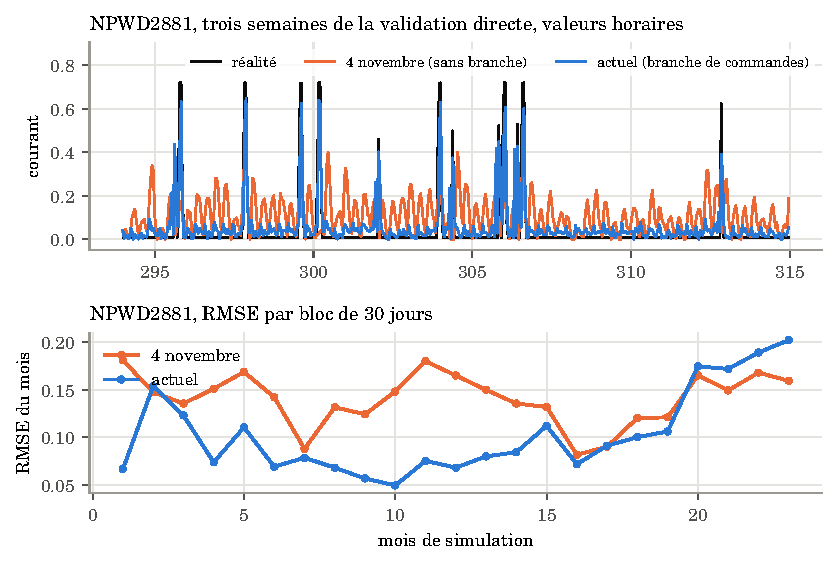
\includegraphics[width=\linewidth]{figures_8_novembre/npwd2881.pdf}
\caption{NPWD2881 en validation directe, avant et après la branche de commandes. En haut, trois semaines (jours 294 à 315, choisis pour la lisibilité) ; en bas, RMSE du circuit par bloc de 30 jours sur toute la simulation.}
\label{fig:npwd2881}
\end{figure}

%=====================================================================
\section{Correction de niveau sur le résidu}

La correction du 4 novembre ajoutait à la sortie l'écart moyen de chaque circuit entre \code{power\_init} et la moyenne d'entraînement. Cet écart contient une part que le contexte explique déjà : si le Soleil est plus proche ou les éclipses plus longues pendant les 7 premiers jours, le simulateur le sait sans aide. La correction comptait donc cette part deux fois.

La nouvelle version (I4) fait tourner le simulateur sur les 7 jours de \code{power\_init}, avec un état nul et sans gradient, et mesure l'écart moyen entre ses prédictions et les vrais courants. Seul ce résidu, que le contexte n'explique pas, passe dans la correction. Il reste borné à $\pm 5$ en unités centrées-réduites, comme avant. La forme $w_c\, r_c\, 2^{-t/\tau_c}$ ne change pas, avec $r_c$ le résidu du circuit $c$.

\begin{table}[!htb]
\centering\small
\caption{Essais sur la correction de niveau et réglages divers (GPU T4). Les lignes grisées sont retenues.}
\label{tab:residu}
\begin{tabularx}{\linewidth}{l X r r r}
\toprule
 & Changement & Directe & Inverse & Moyenne \\
\midrule
I1 & G2b + second terme de correction, demi-vie initiale 180 jours & 0.0835 & 0.0919 & 0.0877 \\
I2 & G2b, 900 pas et moyenne exponentielle 0.995 & 0.0838 & 0.0929 & 0.0884 \\
I3 & G2b, 10 graines par membre au lieu de 5 & 0.0835 & 0.0908 & 0.0872 \\
\rowcolor{fond} \textbf{I4} & \textbf{G2b + correction sur le résidu (retenu)} & \textbf{0.0829} & \textbf{0.0901} & \textbf{0.0865} \\
I5 & G2b, lots de 64 épisodes & 0.0834 & 0.0920 & 0.0877 \\
I7 & G2b, taux d'apprentissage $2\cdot10^{-3}$ & 0.0833 & 0.0918 & 0.0876 \\
K1 & I4 + cibles de la branche choisies sur l'entraînement & 0.0821 & 0.0901 & 0.0861 \\
\rowcolor{fond} \textbf{L1} & \textbf{I4 + second terme lent, sur le résidu (retenu)} & \textbf{0.0827} & \textbf{0.0892} & \textbf{0.0859} \\
L2 & I4, GRU de 192 unités au lieu de 128 & 0.0829 & 0.0911 & 0.0870 \\
M1 & I4, l'encodeur lit aussi le résidu heure par heure & 0.0831 & 0.0898 & 0.0865 \\
M2 & I4, morceaux de 60 jours au lieu de 30 & 0.0827 & 0.0900 & 0.0863 \\
N4 & L1, dropout 0.2 & 0.0825 & 0.0893 & 0.0859 \\
N5 & L1, moyenne exponentielle 0.995 & 0.0821 & 0.0897 & 0.0859 \\
\bottomrule
\end{tabularx}
\end{table}

I4 gagne 0.0008 sur les graines 0 à 4 et autant sur les graines 5 à 9, avec les deux directions en baisse à chaque fois. Le gain porte sur les circuits dont le niveau change entre les périodes : en inverse, NPWD2531 passe de 0.240 à 0.229 et NPWD2851 de 0.178 à 0.169.

Un second terme de correction, avec une demi-vie initialisée à 180 jours, n'aidait pas tant que la correction portait sur l'écart à la moyenne (I1 : $+0.0004$). Sur le résidu, il gagne 0.0005 sur les graines 0 à 4 et 0.0003 sur les graines 5 à 9 (L1), toujours dans les deux directions. Le gain est petit, mais il se retrouve dans les quatre mesures ; je l'ai gardé. Le modèle dispose ainsi d'un terme rapide pour les premières semaines et d'un terme lent pour les décalages qui durent plusieurs mois.

Le choix automatique des cibles de la branche (J1, K1, N1) mérite une remarque. La règle retient les circuits dont la corrélation maximale avec une variable de commande dépasse 0.5 sur l'entraînement. Sur annee1, elle ajoute NPWD2531 ; sur annee2, elle ne garde que NPWD2881, donc l'inverse ne change pas. Le gain moyen est resté entre 0.0003 et 0.0004 sur trois mesures, sous le seuil de 0.0005 : non retenu. Plus de pas, plus de graines, un réseau plus grand ou des lots plus gros n'ont rien apporté non plus. Après L1, six essais de suite sans gain ont clos la session à 0.0827 / 0.0892 / 0.0859.

%=====================================================================
\section{Robustesse temporelle et borne du résidu}

\subsection{Diagnostic}

L'outil \code{outils/diagnostic\_temporel.py} découpe l'erreur par circuit, par bloc de 30 jours, par régime de consommation (seuils aux quantiles 50 et 90 de l'entraînement) et selon la présence de commandes inconnues ou de modes de pointage rares. Quatre constats en sont sortis.

\begin{itemize}
  \item En inverse, NPWD2531 est le deuxième contributeur à l'erreur. Son écart-type prédit vaut 0.069 contre 0.241 observé : le modèle aplatit ce circuit.
  \item Son résidu initial normalisé vaut entre 6.96 et 7.45 selon le membre et la graine. La borne de 5 en coupait donc une partie.
  \item Les heures sans mesure \code{saaf} représentent 1.6 \% des cellules de la directe et 1.9 \% de l'erreur quadratique. La couverture \code{saaf} moyenne vaut 1.000 sur annee1 et 0.802 sur annee2.
  \item Les commandes inconnues et les modes rares ne montrent pas de dégradation systématique. Je n'ai pas repris les rattachements de commandes déjà rejetés.
\end{itemize}

\subsection{Essais}

Trois essais ont été réentraînés et rejetés (tableau~\ref{tab:robustesse}). Des épisodes de durée variable, entre 30 et 365 jours, dégradent les deux directions et 17 des 24 fenêtres temporelles testées. Une borne de 10 dès l'entraînement améliore NPWD2531 en inverse mais le dégrade en directe. Un plancher de 0.01 sur l'échelle du résidu, pensé pour limiter le bruit des circuits presque constants, dégrade l'inverse.

\begin{table}[!htb]
\centering\small
\caption{Session « robustesse temporelle » (graines 0 à 4). Les RMSE sont données à $10^{-6}$ près, car certains écarts sont très faibles.}
\label{tab:robustesse}
\begin{tabularx}{\linewidth}{X r r r l}
\toprule
Essai & Directe & Inverse & Moyenne & Décision \\
\midrule
Référence (L1, GPU) & 0.082651 & 0.089233 & 0.085942 & -- \\
Épisodes de 30 à 365 jours & 0.083285 & 0.090783 & 0.087034 & rejet \\
Borne 10 dès l'entraînement & 0.083008 & 0.088280 & 0.085644 & rejet (directe) \\
Plancher d'échelle du résidu à 0.01 & 0.082504 & 0.089474 & 0.085989 & rejet (inverse) \\
\rowcolor{fond} \textbf{Borne 10 à la prédiction seulement} & \textbf{0.082651} & \textbf{0.088056} & \textbf{0.085354} & \textbf{retenu} \\
\bottomrule
\end{tabularx}
\end{table}

La correction retenue ne touche pas l'entraînement. À la prédiction, la borne du résidu passe de 5 à 10 pour les circuits dont l'écart-type d'entraînement atteint 0.01 ; les autres gardent la borne 5, car leur faible écart-type peut produire des résidus normalisés de plusieurs centaines. Aucun nom de circuit n'intervient dans ce choix, et le seuil 0.01 est celui que le code utilisait déjà pour repérer les circuits variables. Les poids sont les mêmes que ceux de la référence : la directe donne des fichiers identiques, l'inverse gagne 0.0012 sur les graines 0 à 4 et 0.0010 sur les graines 5 à 9.

La figure~\ref{fig:niveau} reprend NPWD2531 en validation inverse. Sur les 90 premiers jours, sa RMSE passe de 0.527 sans correction à 0.447 avec la correction du 4 novembre, puis à 0.349 avec le résidu et la borne 10. Sur toute la période, elle passe de 0.263 à 0.241 puis à 0.208. Au début de la simulation, le modèle prédit environ 0.43 pour une valeur réelle proche de 0.6. La correction décroît ensuite alors que le circuit reste haut jusqu'au jour 140.

\begin{figure}[!htb]
\centering
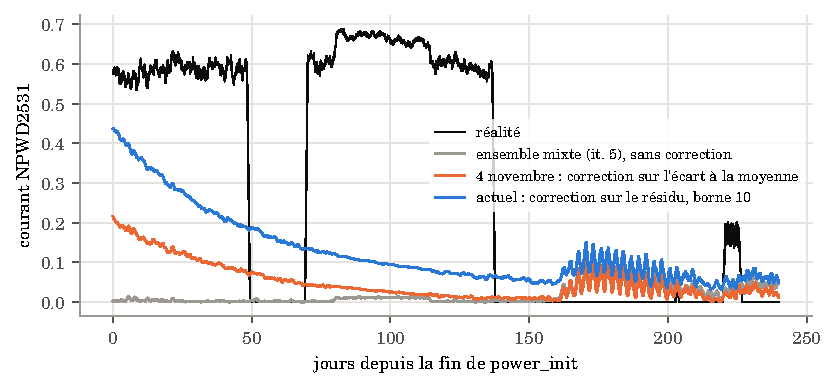
\includegraphics[width=\linewidth]{figures_8_novembre/niveau.pdf}
\caption{NPWD2531 pendant les 240 premiers jours de la validation inverse (moyennes glissantes sur 24 h). Trois versions de la correction de niveau.}
\label{fig:niveau}
\end{figure}

\subsection{Stabilité selon le point de départ}

Les deux validations officielles démarrent toujours au premier jour de la période. Pour savoir si la borne 10 aide aussi à d'autres moments, j'ai lancé des simulations depuis les jours 0, 120, 300 et 480 de la période tenue hors apprentissage, avec 168 heures de démarrage et des horizons de 30, 90 et 365 jours, soit 12 fenêtres par direction.

\begin{table}[!htb]
\centering\small
\caption{Moyenne et pire valeur des 12 RMSE de fenêtre, avant et après la borne 10.}
\label{tab:fenetres}
\begin{tabular}{l l r r r r}
\toprule
 & & \multicolumn{2}{c}{Moyenne des 12} & \multicolumn{2}{c}{Pire fenêtre} \\
Graines & Direction & référence & borne 10 & référence & borne 10 \\
\midrule
0--4 & directe & 0.074651 & 0.074619 & 0.098765 & 0.098579 \\
0--4 & inverse & 0.086007 & 0.084414 & 0.100398 & 0.094779 \\
5--9 & directe & 0.074716 & 0.074677 & 0.097292 & 0.097050 \\
5--9 & inverse & 0.086012 & 0.084282 & 0.103197 & 0.097740 \\
\bottomrule
\end{tabular}
\end{table}

En inverse, 4 fenêtres s'améliorent, 6 ne changent pas et 2 se dégradent dans chaque groupe de graines. Les deux régressions concernent le départ au jour 120, sur 90 et 365 jours ($+0.0017$ et $+0.0006$ sur les graines 0 à 4). Le gain n'est donc pas universel : il vient surtout de l'adaptation initiale en inverse. Ces fenêtres se chevauchent et ne sont pas des mesures indépendantes.

%=====================================================================
\section{Régularisations de robustesse}

La validation ne couvre que deux situations. Deux changements de distribution me paraissent plausibles : une longue lacune de télémétrie \code{saaf}, comme celles d'annee2, et un changement dans la façon dont les états AOOO/ATTT sont codés. J'ai ajouté deux régularisations pour que le modèle y soit moins sensible.

\paragraph{Masquage \code{saaf} par blocs.} Chaque période d'entraînement est gardée et reçoit une copie dans laquelle 10 \% des heures, en blocs de 1 à 720 heures (longueur tirée en log-uniforme), ont les colonnes \code{saaf} remplacées par les valeurs d'une vraie lacune : valeurs de remplissage du schéma, couverture à 0, indicateur de manque à 1. Le masque est fixe pour une période donnée. Les statistiques de normalisation et le choix des variables sont calculés sur les périodes d'origine.

\paragraph{Abandon groupé des états.} Pendant l'entraînement, avec une probabilité de 0.5 par épisode, les 38 variables d'état des commandes sont mises à 0 sur tout l'épisode, après normalisation. Les impulsions restent intactes. La branche vers NPWD2881 ne peut donc pas dépendre d'un code d'état exact. Rien n'est masqué à la prédiction.

\begin{table}[!htb]
\centering\small
\caption{Régularisations de robustesse (GPU T4, PyTorch 2.15). La référence est la configuration avec borne 10, relancée dans le même environnement.}
\label{tab:regularisations}
\begin{tabularx}{\linewidth}{l X r r r}
\toprule
Graines & Configuration & Directe & Inverse & Moyenne \\
\midrule
0--4 & référence & 0.082650 & 0.088082 & 0.085366 \\
0--4 & masquage \code{saaf} 0.1 + abandon des états 0.5 & 0.082553 & 0.088474 & 0.085513 \\
5--9 & référence & 0.083092 & 0.088354 & 0.085723 \\
\rowcolor{fond} 5--9 & \textbf{masquage \code{saaf} 0.1 + abandon des états 0.5 (retenu)} & \textbf{0.083361} & \textbf{0.088258} & \textbf{0.085810} \\
\bottomrule
\end{tabularx}
\end{table}

Pour cette session, le critère était différent : aucune direction dégradée de plus de 0.0005 et une moyenne au plus égale à 0.08587. Le candidat le respecte dans les deux groupes. Il n'améliore pas la validation : la direction qui se dégrade change d'un groupe à l'autre, et les écarts ($+0.00015$ et $+0.00009$ sur la moyenne) restent sous le bruit de graine. Je l'ai gardé pour la robustesse attendue. Ce gain n'est pas mesuré, puisqu'aucune validation ne contient de lacune \code{saaf} artificielle ou d'états recodés. C'est un pari, et il coûte environ 0.0001.

Les deux options valent 0 par défaut. Avec les options à 0, un petit entraînement donne des poids identiques au bit près à ceux du code précédent, et les anciens poids se rechargent sans changement.

%=====================================================================
\section{Tête de régime partagée (non retenue)}

\subsection{Motivation}

NPWD2551 et NPWD2451 font 55 \% de l'erreur quadratique de la directe et n'ont presque pas bougé depuis le 4 novembre. L'outil \code{outils/diagnostic\_regimes.py} montre que ces circuits alternent entre deux niveaux. NPWD2551 vaut 0.0006 en régime bas et 0.585 en régime haut sur annee1, avec 47.6 \% des heures en régime haut. Il change de régime 5.6 fois par jour ; un passage bas dure 4 heures en médiane, un passage haut 2 heures. NPWD2451 change 4.8 fois par jour. NPWD2851 change beaucoup moins souvent sur annee1 (0.5 fois par jour) mais 4.9 fois par jour sur annee2.

Avec une perte quadratique, un modèle qui ne sait pas dans quel régime se trouve le circuit prédit une valeur intermédiaire. L'idée était de lui donner une variable qui représente explicitement ce régime.

\subsection{Dispositif}

L'option \code{regime\_partage} ajoute au simulateur une tête qui donne, à chaque heure, une probabilité de régime commune à NPWD2551, NPWD2451 et NPWD2851, et un niveau par circuit et par régime. La sortie de ces trois circuits devient l'espérance du mélange. Les seuils de régime sont appris par k-moyennes sur le logarithme des courants d'entraînement. Une entropie croisée pondérée, de poids $\lambda$, s'ajoute à la perte ; son gradient ne remonte pas dans le GRU, pour ne pas déformer l'état du simulateur. Deux options l'accompagnent : \code{abandon\_regime\_contexte}, qui masque des blocs d'éclipses, de modes de pointage et de commandes pendant l'entraînement, et \code{curriculum\_jours}, qui allonge les épisodes au fil des pas.

\subsection{Résultats}

\begin{table}[!htb]
\centering\small
\caption{Tête de régime et variantes. Criblage sur une graine, puis confirmation sur cinq graines. La référence inclut les régularisations de la section 5.}
\label{tab:regimes}
\begin{tabularx}{\linewidth}{l X r r r}
\toprule
Graines & Changement & Directe & Inverse & Moyenne \\
\midrule
0 & référence & 0.08335 & 0.08956 & 0.08646 \\
0 & tête de régime, $\lambda = 0.02$ & 0.08372 & 0.08984 & 0.08678 \\
0 & tête de régime, $\lambda = 0.05$ & 0.08370 & 0.08968 & 0.08669 \\
0 & tête de régime, $\lambda = 0.1$ & 0.08382 & 0.09013 & 0.08697 \\
0 & masquage du contexte 0.1 & 0.08360 & 0.08935 & 0.08647 \\
0 & curriculum 180, 365 puis 540 jours & 0.08313 & 0.09038 & 0.08675 \\
0 & épisodes de 540 jours & 0.08439 & 0.08789 & 0.08614 \\
\midrule
0--4 & référence & 0.08255 & 0.08847 & 0.08551 \\
0--4 & tête de régime, $\lambda = 0.05$ & 0.08350 & 0.08903 & 0.08626 \\
0--4 & tête de régime, $\lambda = 0.05$ + masquage du contexte 0.1 & 0.08349 & 0.08865 & 0.08607 \\
0--4 & épisodes de 540 jours & 0.08420 & 0.08776 & 0.08598 \\
\bottomrule
\end{tabularx}
\end{table}

Aucune variante ne bat la référence. La meilleure combinaison (tête de régime et masquage du contexte) perd 0.0009 en directe et 0.0002 en inverse. La tête apprend pourtant quelque chose sur le régime : son score de Brier vaut 0.150 en directe, contre 0.219 pour une probabilité constante égale à la fréquence d'entraînement, et 0.183 contre 0.247 en inverse. La figure~\ref{fig:regimes} montre que sa calibration se décale d'une période à l'autre. En directe, elle sous-estime la part de régime haut (67.5 \% observé, 59.9 \% prédit en moyenne) ; en inverse, elle la surestime (44.2 \% observé, 52.0 \% prédit). Savoir mieux classer le régime ne suffit pas à baisser la RMSE quand la proportion de régime haut change entre les périodes.

\begin{figure}[!htb]
\centering
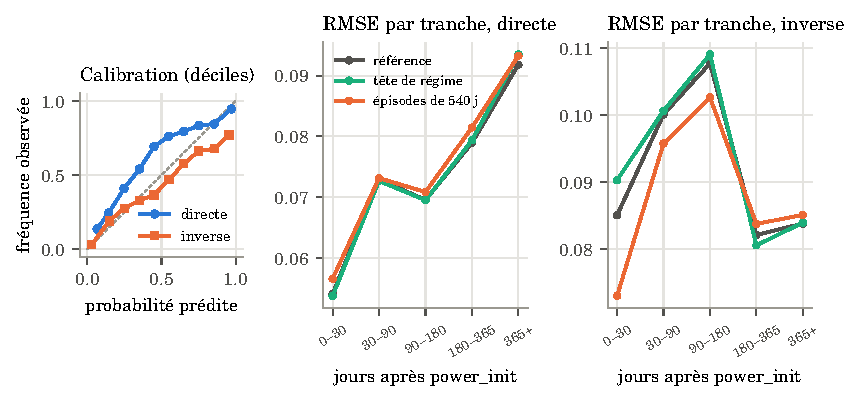
\includegraphics[width=\linewidth]{figures_8_novembre/regimes.pdf}
\caption{À gauche, calibration de la probabilité de régime haut (tête de régime + masquage du contexte, cinq graines), par décile de probabilité prédite. Au centre et à droite, RMSE globale par tranche d'horizon pour la référence et deux candidats.}
\label{fig:regimes}
\end{figure}

Les épisodes de 540 jours donnent le résultat le plus net, dans des sens opposés selon la direction : l'inverse gagne 0.0007 et la directe perd 0.0016. En inverse, le gain porte sur les six premiers mois (0.073 contre 0.085 sur le premier) ; en directe, la perte se répartit sur toute la période. Une seule période de 687 jours ne laisse que 140 jours de départs possibles pour un épisode de 547 jours. Je pense que ce manque de diversité explique l'instabilité, sans l'avoir vérifié.

{\sloppy Les options restent dans \code{dio/monde.py}, coupées par défaut, et leurs tests dans \code{tests/test\_regime.py}. Le dossier \code{poids\_candidats/regime\_partage/} garde les poids du candidat ; ils ne servent pas à la prédiction.\par}

%=====================================================================
\section{Résultats du modèle actuel}

\subsection{Score global}

\begin{table}[!htb]
\centering\small
\caption{RMSE sur les deux validations. « Actuel » désigne la configuration de \code{poids/} entraînée sur une seule période par direction (\code{runs/rob\_cand\_g04}).}
\label{tab:final}
\begin{tabular}{l r r r r}
\toprule
Modèle & Directe & Inverse & Moyenne & Gain vs constante \\
\midrule
Constante & 0.1058 & 0.1252 & 0.1155 & -- \\
Gradient boosting + recalage & 0.0951 & 0.0999 & 0.0975 & $-15.6$ \% \\
World model du 4 novembre & 0.0853 & 0.0940 & 0.0897 & $-22.3$ \% \\
\textbf{World model actuel} & \textbf{0.0826} & \textbf{0.0885} & \textbf{0.0855} & $\mathbf{-26.0}$ \% \\
\bottomrule
\end{tabular}
\end{table}

En quatre jours, la moyenne a baissé de 0.0042. L'inverse gagne plus que la directe (0.0055 contre 0.0027), ce qui correspond à l'effet attendu des corrections de niveau. La figure~\ref{fig:progression} détaille la contribution de chaque étape. Le meilleur score mesuré (0.08535) date d'avant les régularisations de robustesse.

\begin{figure}[!htb]
\centering
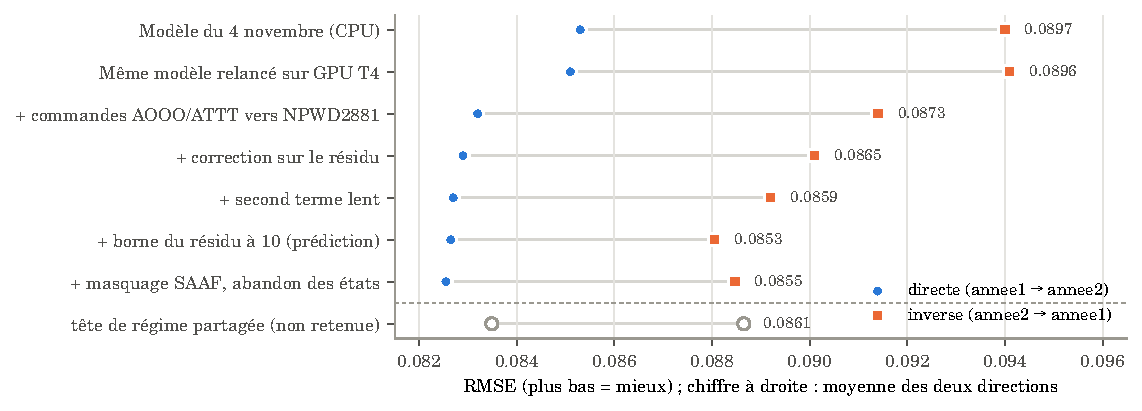
\includegraphics[width=\linewidth]{figures_8_novembre/progression.pdf}
\caption{Progression depuis le 4 novembre. Chaque ligne relie la RMSE directe (rond) et la RMSE inverse (carré) d'une configuration. La dernière ligne, en creux, est le candidat non retenu de la section 6.}
\label{fig:progression}
\end{figure}

\subsection{Dérive sur la période simulée}

La figure~\ref{fig:derive} reprend la courbe de dérive du premier rapport. Le modèle actuel fait mieux que celui du 4 novembre sur 17 blocs sur 23 en directe et 20 sur 23 en inverse. Il bat la constante sur 22 blocs en directe et sur les 23 en inverse. Le gain le plus fort est au début de l'inverse : 0.085 contre 0.112 sur le premier mois, puis 0.090 contre 0.103 sur le deuxième. C'est la période où la correction de niveau agit. Les pics des mois difficiles (8\textsuperscript{e} mois en directe, 4\textsuperscript{e} en inverse) restent presque à la même hauteur.

\begin{figure}[!htb]
\centering
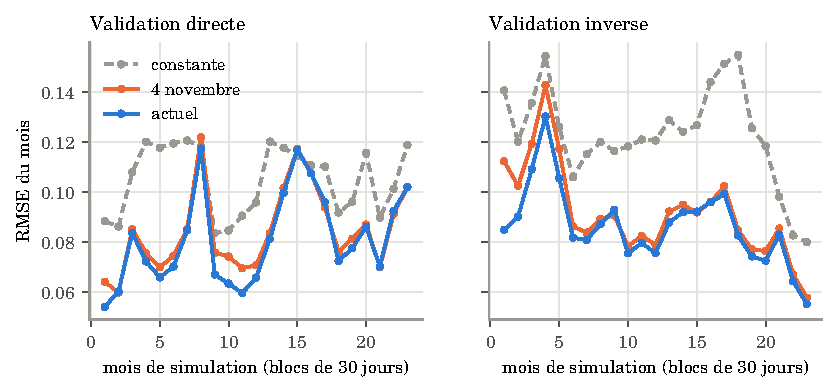
\includegraphics[width=\linewidth]{figures_8_novembre/derive.pdf}
\caption{RMSE par bloc de 30 jours après la fin de \code{power\_init}, pour la constante, le modèle du 4 novembre et le modèle actuel.}
\label{fig:derive}
\end{figure}

\subsection{Erreurs par circuit}

\begin{figure}[!htb]
\centering
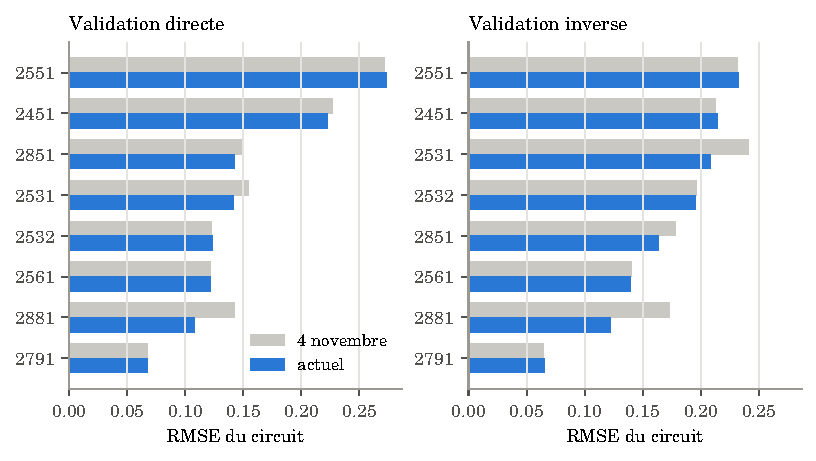
\includegraphics[width=\linewidth]{figures_8_novembre/circuits.pdf}
\caption{RMSE par circuit pour les huit circuits qui contribuent le plus à l'erreur du modèle actuel (préfixe NPWD omis).}
\label{fig:circuits}
\end{figure}

Le gain vient de trois circuits (figure~\ref{fig:circuits}). NPWD2881 passe de 0.143 à 0.108 en directe et de 0.173 à 0.122 en inverse ; il fait maintenant mieux que la constante apprise sur annee1 (0.124). NPWD2531 passe de 0.154 à 0.141 en directe et de 0.241 à 0.208 en inverse, mais reste un peu au-dessus de cette constante en directe (0.138). NPWD2851 gagne 0.006 en directe et 0.014 en inverse.

Les deux plus gros contributeurs ne bougent pas : NPWD2551 passe de 0.271 à 0.273 en directe et NPWD2451 de 0.227 à 0.223. Ils pèsent maintenant 33 \% et 22 \% de l'erreur quadratique de la directe, contre 31 \% et 21 \% au 4 novembre, puisque le reste de l'erreur a baissé. NPWD2532 et NPWD2561 n'ont pas changé non plus.

\subsection{Incertitude}

Sur la validation directe, 76.9 \% des valeurs réelles tombent dans la bande de $\pm 2$ écarts-types de l'ensemble, et 78.7 \% en inverse (77.3 \% et 79.3 \% au 4 novembre). La bande de $\pm 1$ écart-type contient 68.7 \% et 68.5 \% des valeurs, soit presque exactement les 68 \% d'une loi normale. L'écart-type de l'ensemble a donc la bonne échelle pour les erreurs courantes ; ce sont les grandes erreurs qui sont plus fréquentes qu'une loi normale ne le prévoit. Un simple facteur d'échelle ne corrigerait pas les deux bandes à la fois. Ces couvertures sont calculées sur des prédictions refaites sur CPU, qui retrouvent la RMSE du journal en directe (0.082553) et s'en écartent de $2.5\cdot10^{-5}$ en inverse.

\subsection{Ablations}

Les ablations ont été relancées sur la configuration du 5 novembre (membre v1 seul, 2 graines par direction, sur GPU). Elles n'ont pas été refaites après les régularisations de robustesse.

\begin{table}[!htb]
\centering\small
\caption{Ablations (\code{outils/ablations.py}, détail dans \code{docs/ABLATIONS.md}).}
\label{tab:ablations}
\begin{tabular}{l r r r}
\toprule
Variante & Directe & Inverse & Écart moyen vs complet \\
\midrule
complet & 0.0840 & 0.0918 & -- \\
sans éclipses & 0.0844 & 0.0910 & $-0.0002$ \\
sans branche AOOO/ATTT & 0.0857 & 0.0939 & $+0.0019$ \\
sans \code{saaf} (Soleil) & 0.0865 & 0.0950 & $+0.0028$ \\
sans \code{dmop} (comptes et branche) & 0.0885 & 0.0944 & $+0.0035$ \\
sans mémoire & 0.0884 & 0.1032 & $+0.0079$ \\
\bottomrule
\end{tabular}
\end{table}

\begin{figure}[!htb]
\centering
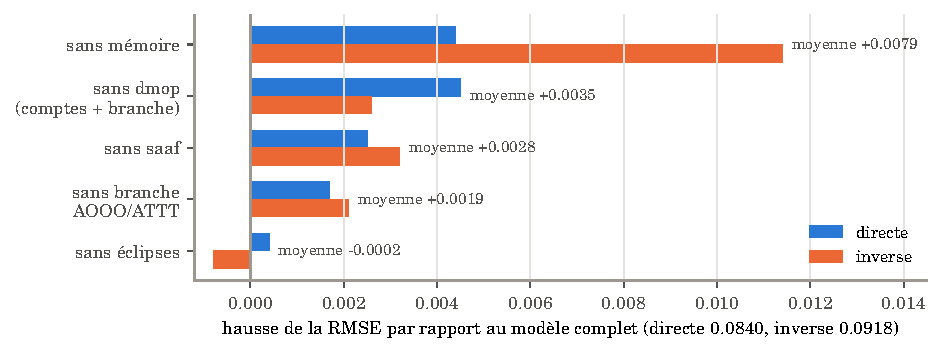
\includegraphics[width=\linewidth]{figures_8_novembre/ablations.pdf}
\caption{Hausse de la RMSE quand on retire un élément du modèle, par direction.}
\label{fig:ablations}
\end{figure}

La mémoire reste l'élément le plus important, surtout en inverse ($+0.0114$). Les commandes \code{dmop} pèsent maintenant 0.0035, contre 0.0019 au 4 novembre, et la branche AOOO/ATTT en représente 0.0019. Les éclipses ne comptent plus ($-0.0002$, sous le bruit de graine), alors qu'elles valaient 0.0016 avant. Mon interprétation : la correction sur le résidu et les variables de saison (\code{saaf}, \code{ltdata}) portent maintenant l'information qu'elles apportaient. Je les garde, puisque les retirer ne fait rien gagner de mesurable.

\subsection{État du dépôt}

Le code a été rangé avant le rendu : \code{dio/} pour le modèle et la préparation, \code{outils/} pour la validation, les ablations, les diagnostics et Kaggle, \code{tests/} et \code{docs/}. Le code des variantes écartées a été retiré ; seules restent, coupées par défaut, les options de la section 6. Les dossiers de validation ne sont plus versionnés ; \code{make\_validation.py} les recrée. La suite compte 40 tests (\code{python -m unittest discover -s tests}), dont la prédiction de bout en bout avec les poids livrés. L'entraînement du modèle final prend 629 s sur GPU T4 et la prédiction 10 s sur CPU ; les poids pèsent 6.9 Mo.

%=====================================================================
\section{Limites et travail restant}

\begin{itemize}
  \item NPWD2551 et NPWD2451 font 55 \% de l'erreur de la directe et n'ont pas progressé depuis le 4 novembre. Ils changent de régime cinq fois par jour environ, et ni le contexte ni la tête de régime n'ont permis de prévoir ces changements dans les deux directions.
  \item La branche de commandes fait plus mal que l'ancien modèle sur NPWD2881 pendant les quatre derniers mois de la directe. La cause n'est pas vérifiée.
  \item NPWD2531 reste aplati : en inverse, le modèle rattrape une grande partie du niveau de départ, mais la correction décroît pendant que le circuit reste haut.
  \item L'incertitude est bien dimensionnée à $\pm 1$ écart-type et trop étroite à $\pm 2$. Il faudrait une loi à queues plus lourdes, ou des quantiles appris, plutôt qu'un facteur d'échelle.
  \item Le gain des régularisations de robustesse n'est pas mesuré. Une validation avec une lacune \code{saaf} artificielle sur la période de test permettrait de le vérifier.
  \item Le bonus pilote n'est pas commencé.
  \item Comme au 4 novembre, l'entraînement final sur annee1 et annee2 fusionnées ne peut pas être validé, faute de période de validation indépendante.
\end{itemize}

%=====================================================================
\appendix
\section{Reproduire les résultats}

Environnement : Python 3.13, \code{uv sync} (ou \code{pip install -r requirements.txt}). Sur Kaggle, \code{outils/lancer\_kaggle.py} lance les mêmes commandes sur GPU T4.

\begin{small}
\begin{verbatim}
python train.py                                   # modèle final -> poids/
python predict.py --test_dir DOSSIER --out predictions.csv
python outils/valider.py --nom essai --options '{"masque_saaf": 0.1, "abandon_etats": 0.5,
    "borne_niveau_prediction": 10.0}'             # directe + inverse
python outils/diagnostic_temporel.py --run runs/essai   # erreurs par circuit et bloc
python outils/diagnostic_regimes.py --donnees          # régimes de 2551, 2451, 2851
python docs/rapport/figures_8_novembre.py --preds DOSSIER     # figures
\end{verbatim}
\end{small}

Le fichier \code{docs/RESULTATS.md} contient le journal complet des essais, avec les durées et les environnements.

\end{document}
